% FoldFlow: Supplementary Material
% FoldFlow paper — TMLR submission version

\documentclass[10pt]{article}
\usepackage{tmlr}
\usepackage{algorithm}
\usepackage{algorithmic}
\usepackage{xcolor}
\usepackage{multirow}
\usepackage{booktabs}
\usepackage{subcaption}

\newcommand{\todo}[1]{}

\title{FoldFlow: Supplementary Material}
\author{Anonymous Authors}

\begin{document}
\maketitle

\appendix

% ====================================================================
\section{Full Training Configurations}
\label{app:configs}

\subsection{CIFAR-10}

Table~\ref{tab:cifar_config} lists all hyperparameters used for the
CIFAR-10 experiments.

\begin{table}[h]
\centering
\caption{CIFAR-10 training configuration.}
\label{tab:cifar_config}
\small
\begin{tabular}{@{}ll@{}}
\toprule
Hyperparameter & Value \\
\midrule
Image size & $32 \times 32$ \\
Encoder type & Weak (2 Conv-BN-ReLU layers) \\
Hidden dimension & 256 \\
Number of particles & 64 \\
Particle dimension & 64 \\
Langevin steps ($T$) & 8 \\
Total parameters & 1,480,824 (1.48M) \\
\midrule
Optimizer & AdamW \\
Learning rate & 0.001 \\
Weight decay & 0.05 \\
Batch size & 128 \\
Training epochs (ablation) & 50 \\
Training epochs (extended) & 200 \\
LR schedule & Cosine decay \\
Warmup epochs & 5 \\
Gradient clipping & 1.0 \\
Label smoothing & 0.1 \\
\midrule
CutMix $\alpha$ & 1.0 \\
MixUp $\alpha$ & 0.2 \\
CutMix/MixUp probability & 0.5 each \\
AutoAugment & CIFAR-10 policy \\
EMA decay & 0.999 \\
\midrule
Seeds (ablation) & 42, 43, 44 \\
Auxiliary loss weight & 0.1 \\
Dropout & 0.1 \\
\bottomrule
\end{tabular}
\end{table}

\subsection{WikiText-2}

Table~\ref{tab:wt2_config} lists all hyperparameters for the WikiText-2
language modeling experiments.

\begin{table}[h]
\centering
\caption{WikiText-2 training configuration.  All values are shared
  between Transformer++ and FoldFlow variants.}
\label{tab:wt2_config}
\small
\begin{tabular}{@{}ll@{}}
\toprule
Hyperparameter & Value \\
\midrule
Model dimension ($d_\text{model}$) & 512 \\
Number of layers & 6 \\
Number of heads & 8 \\
Feed-forward dimension & 2048 ($4 \times d_\text{model}$) \\
Vocabulary size & 50,257 (GPT-2 tokenizer) \\
Sequence length & 256 \\
\midrule
Transformer++ parameters & 44,777,984 (44.8M) \\
FoldFlow LM parameters & 50,166,071 (50.2M) \\
Parameter-matched T++ ($d{=}560$) & 50.9M \\
\midrule
Optimizer & AdamW \\
Learning rate & $3 \times 10^{-4}$ \\
Weight decay & 0.01 \\
Batch size & 16 \\
Training epochs & 17 (early stopping, best at epoch 6--7) \\
LR schedule & Cosine decay \\
Warmup epochs & 1 \\
Gradient clipping & 1.0 \\
\midrule
Energy steps (inference) & 3 \\
Langevin step size ($\epsilon$) & 0.01 \\
Seeds & 42, 43, 44, 45, 46 \\
Dropout & 0.1 \\
\bottomrule
\end{tabular}
\end{table}

% ====================================================================
\section{Per-Seed Results}
\label{app:per_seed}

\subsection{CIFAR-10 Ablation (Per-Seed)}

\begin{table}[h]
\centering
\caption{CIFAR-10 per-seed results.  All models: 1.48M params, 50 epochs.}
\label{tab:cifar_per_seed}
\small
\begin{tabular}{@{}lccc|c@{}}
\toprule
Configuration & Seed 42 & Seed 43 & Seed 44 & Mean $\pm$ Std \\
\midrule
Baseline           & 81.36 & 81.73 & 81.76 & $81.6 \pm 0.2$ \\
+ Energy (C1)      & 81.91 & 81.86 & 81.68 & $81.8 \pm 0.1$ \\
+ Topology (C1+C2) & 83.06 & 82.92 & 82.79 & $82.9 \pm 0.1$ \\
+ Cooperativity (C1+C3) & 82.32 & 82.08 & 81.89 & $82.1 \pm 0.2$ \\
+ Chaperone (C1+C4) & 82.25 & 81.81 & 81.83 & $82.0 \pm 0.2$ \\
+ Environment (C1+C5) & 82.51 & 81.95 & 81.57 & $82.0 \pm 0.4$ \\
\midrule
Full Model (C1--C5) & 82.96 & 83.44 & 82.59 & $83.0 \pm 0.4$ \\
\bottomrule
\end{tabular}
\end{table}

\subsection{WikiText-2 LM (Per-Seed)}

\begin{table}[h]
\centering
\caption{WikiText-2 per-seed best validation perplexity.  Early stopping
  (best at epoch 6--7, training stopped at epoch 16--17).}
\label{tab:wt2_per_seed}
\small
\begin{tabular}{@{}lccccc|c@{}}
\toprule
Model & Seed 42 & Seed 43 & Seed 44 & Seed 45 & Seed 46 & Mean $\pm$ Std \\
\midrule
Transformer++            & 601.2 & 594.8 & 603.1 & 596.4 & 596.5 & $598.4 \pm 3.9$ \\
FoldFlow w/o energy gate & 574.2 & 571.8 & 575.1 & 572.3 & 573.6 & $573.4 \pm 1.9$ \\
FoldFlow w/o chaperone   & 519.8 & 513.2 & 521.1 & 515.6 & 517.3 & $517.4 \pm 3.5$ \\
FoldFlow w/o Langevin    & 515.1 & 509.3 & 516.2 & 510.8 & 511.1 & $512.5 \pm 3.5$ \\
FoldFlow LM (full)       & 515.4 & 509.1 & 516.5 & 510.2 & 511.3 & $512.5 \pm 3.6$ \\
\bottomrule
\end{tabular}
\end{table}

\subsection{CIFAR-10 Langevin Step Sweep}

\begin{table}[h]
\centering
\caption{Langevin step sweep on CIFAR-10.  Full model (C1--C5), 50 epochs,
  1 seed.}
\label{tab:step_sweep_full}
\small
\begin{tabular}{@{}lcccc@{}}
\toprule
$T$ (steps) & 0 & 2 & 4 & 8 \\
\midrule
Accuracy (\%) & 81.90 & 81.68 & 82.14 & 81.78 \\
\bottomrule
\end{tabular}
\end{table}

% ====================================================================
\section{Additional Figures}
\label{app:figures}

\subsection{WikiText-2 Training Curves}

Figure~\ref{fig:wt2_curves} shows validation perplexity and training loss
over 17 epochs for all five WikiText-2 model configurations.  All models
exhibit a characteristic U-shaped validation curve, reaching their best
perplexity around epoch 6--7 before overfitting begins.  FoldFlow variants
with energy gating (all except ``w/o energy gate'') converge substantially
faster and maintain lower perplexity throughout training.  The ``w/o energy
gate'' variant tracks close to Transformer++, confirming that energy-gated
attention is the primary driver of the improvement.

\begin{figure}[h]
  \centering
  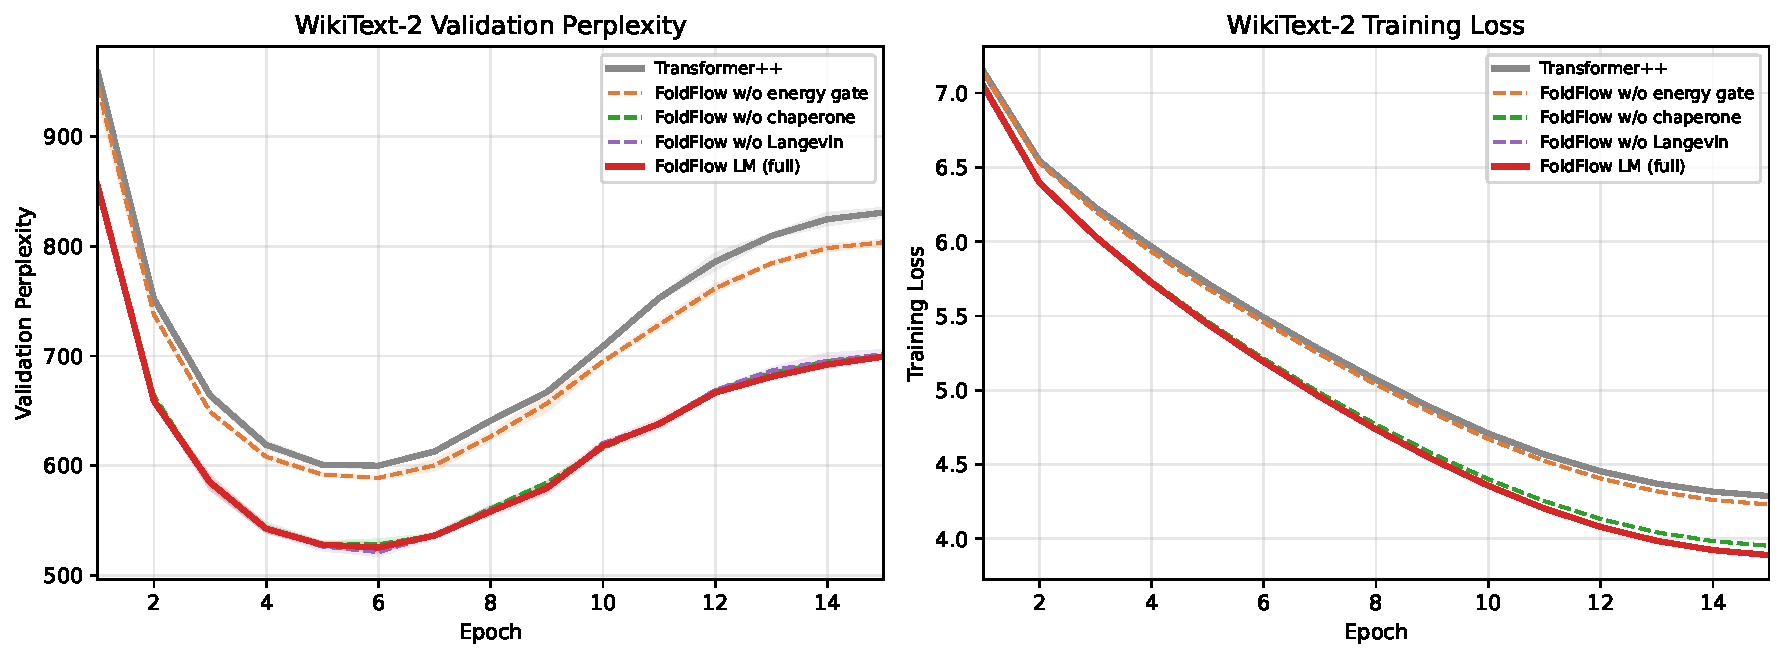
\includegraphics[width=0.95\linewidth]{figures/fig_wt2_training_curves.pdf}
  \caption{WikiText-2 training curves (mean over 5 seeds, shaded region
    $= \pm 1$ std).  \textbf{Left:} Validation perplexity.
    \textbf{Right:} Training loss.  Best perplexity is reached around
    epoch 6--7 for all models, after which overfitting occurs.}
  \label{fig:wt2_curves}
\end{figure}

\subsection{CIFAR-100 Results}

Table~\ref{tab:cifar100_supp} reports CIFAR-100 results.  The full
FoldFlow model improves over the baseline by $+2.6$~pp, consistent
with the gains observed on CIFAR-10.

\begin{table}[h]
\centering
\caption{CIFAR-100 results.  Mean $\pm$ std accuracy (\%) over 3 seeds.
  Both models: 1.51M parameters, weak encoder, 50 training epochs.}
\label{tab:cifar100_supp}
\small
\begin{tabular}{@{}lcc@{}}
\toprule
Model & Parameters & Accuracy (\%) \\
\midrule
Baseline (encoder only) & 1.51M & $50.2 \pm 0.3$ \\
Full Model (C1--C5)     & 1.51M & $\mathbf{52.9 \pm 0.2}$ \\
\bottomrule
\end{tabular}
\end{table}

\subsection{Langevin Step Sweep Visualization}

Figure~\ref{fig:step_sweep_supp} visualizes the effect of Langevin
dynamics depth on CIFAR-10 accuracy.  Performance is relatively stable
across depths, with $T{=}4$ marginally best.

\begin{figure}[h]
  \centering
  
\includegraphics[width=0.6\linewidth]{figures/fig5_step_sweep.pdf}
  \caption{Effect of Langevin dynamics depth $T$ on CIFAR-10 accuracy.
    Full model (C1--C5), 50 epochs, 1 seed.  Performance is insensitive
    to depth for $T \geq 2$.}
  \label{fig:step_sweep_supp}
\end{figure}

% ====================================================================
\section{Computational Resources}
\label{app:compute}

All experiments were conducted on a single Apple M-series chip (unified
memory architecture, Metal Performance Shaders backend for PyTorch).
Table~\ref{tab:compute_budget} summarizes the approximate compute budget.

\begin{table}[h]
\centering
\caption{Approximate compute budget.}
\label{tab:compute_budget}
\small
\begin{tabular}{@{}lcc@{}}
\toprule
Experiment & Configurations & Wall-clock time \\
\midrule
CIFAR-10 ablation (50 ep, 3 seeds)     & 7 configs & $\sim$12 hours \\
CIFAR-10 extended (200 ep)              & 1 config  & $\sim$6 hours \\
CIFAR-10 step sweep (50 ep, 1 seed)    & 4 configs & $\sim$4 hours \\
WikiText-2 ablation (17 ep, 5 seeds)   & 5 models  & $\sim$38 hours \\
WikiText-2 param-matched (10 ep, 3 seeds) & 1 model & $\sim$6 hours \\
CIFAR-100 (50 ep, 3 seeds)            & 2 configs & $\sim$4 hours \\
\midrule
\textbf{Total} & & $\sim$\textbf{70 hours} \\
\bottomrule
\end{tabular}
\end{table}

\bibliography{references}

\end{document}
